% !TEX TS-program = pdflatex
% !TEX encoding = UTF-8 Unicode

\documentclass[a4paper, titlepage=false, parskip=full-, 10pt]{scrartcl}

\usepackage[utf8]{inputenc}
\usepackage[T1]{fontenc}
\usepackage[english, ngerman]{babel}
\usepackage{babelbib}
\usepackage{hyperref}
\usepackage{listings}
\usepackage{framed}
\usepackage{color}
\usepackage{graphicx}
\usepackage[normalem]{ulem}
\usepackage{cancel}
\usepackage{amsmath}
\usepackage{amssymb}
\usepackage{amsthm}
\usepackage{algorithm}
\usepackage{algorithmic}
\usepackage{geometry}
\usepackage{subfigure}
\geometry{a4paper, top=20mm, left=25mm, right=20mm, bottom=40mm}

\newcounter{tasknbr}
\setcounter{tasknbr}{1}
\newenvironment{task}[1]{{\bf Aufgabe \arabic {tasknbr}\stepcounter{tasknbr}} (#1):\begin{enumerate}}{\end{enumerate}}
\newcommand{\subtask}[1]{\item[#1)]}

% Listings -----------------------------------------------------------------------------
\definecolor{red}{rgb}{.8,.1,.2}
\definecolor{blue}{rgb}{.2,.3,.7}
\definecolor{lightyellow}{rgb}{1.,1.,.97}
\definecolor{gray}{rgb}{.7,.7,.7}
\definecolor{darkgreen}{rgb}{0,.5,.1}
\definecolor{darkyellow}{rgb}{1.,.7,.3}
\lstloadlanguages{C++,[Objective]C,Java}
\lstset{
escapeinside={§§}{§§},
basicstyle=\ttfamily\footnotesize\mdseries,
columns=fullflexible,
keywordstyle=\bfseries\color{blue},
commentstyle=\color{darkgreen},      
stringstyle=\color{red},
numbers=left,
numberstyle=\ttfamily\scriptsize\color{gray},
breaklines=true,
showstringspaces=false,
tabsize=4,
captionpos=b,
float=htb,
frame=tb,
frameshape={RYR}{y}{y}{RYR},
rulecolor=\color{black},
xleftmargin=15pt,
xrightmargin=4pt,
aboveskip=\bigskipamount,
belowskip=\bigskipamount,
backgroundcolor=\color{lightyellow},
extendedchars=true,
belowcaptionskip=15pt}

%% Enter current values here: %%
\newcommand{\lecture}{Computer Vision WS15/16}
\newcommand{\tutor}{}
\newcommand{\assignmentnbr}{3}
\newcommand{\students}{Julius Auer}
%%-------------------------------------%%

\begin{document}  
{\small \textsl{\lecture \hfill \tutor}}
\hrule
\begin{center}
\textbf{Übungsblatt \assignmentnbr}\\
[\bigskipamount]
{\small \students}
\end{center}
\hrule

Ich bin so frei, die Aufgabenstellung ein wenig zu interpretieren:

- da CAMSHIFT für ein Einzelbild wenig Sinn macht, werde ich eine Folge von Frames aus dem avi untersuchen (die Änderung der Fenstergröße bei CAMSHIFT ist sonst nicht gut zu sehen)\\
- einige Optimierungen aus dem Paper sind speziell für ''Fleisch'' vorgenommen worden und sollten für das Auto neu untersucht werden (Fehlerfunktion für Histogramm und Funktion zur Anpassung der Fenstergröße)

Ich löse die Aufgaben somit in Hinblick auf eine gute CAMSHIFT-Implementierung, die für das avi brauchbare Ergebnisse liefert - Fleisch ist dort nunmal eher wenig zu sehen ...

\begin{task}{Farbräume}
\subtask{1.1}
\emph{- Lade das angehängte Bild ''racecar.png''\\
- konvertiere das Bild in den HSV-Farbraum\\
- stelle das Histogramm über dem Hue-Kanal für das gesamte Bild dar}

\begin{figure}[!htpb]
\centering
\subfigure[Original]{
  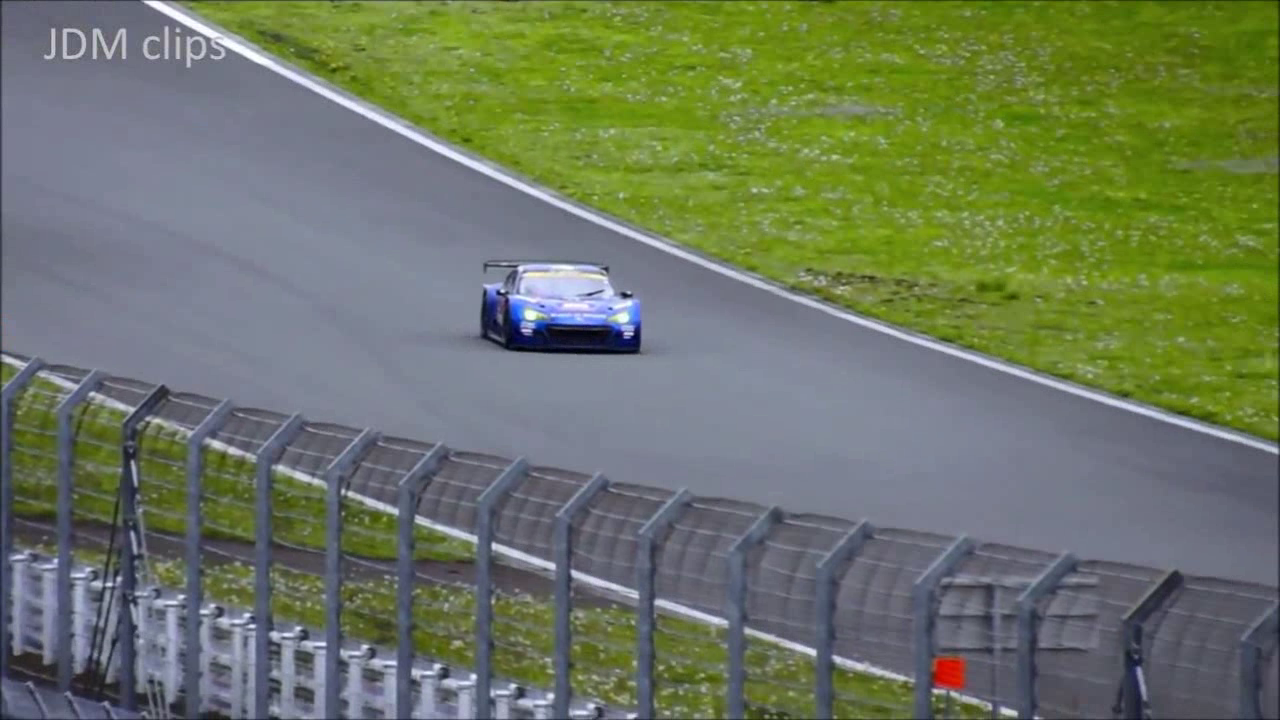
\includegraphics[width=0.48\linewidth]{racecar}
}
\subfigure[Hue]{
  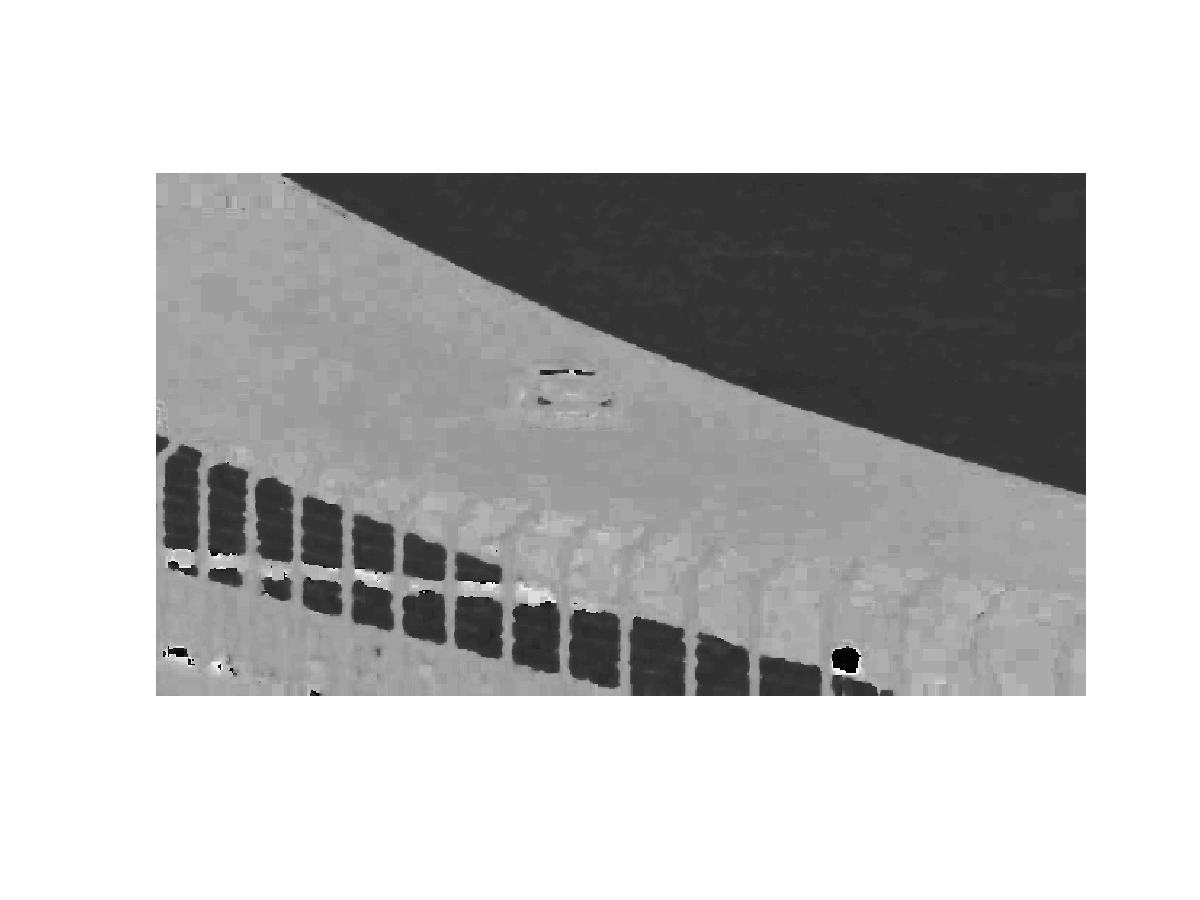
\includegraphics[width=0.48\linewidth]{generated/hsv_h}
}
\subfigure[Satuation]{
  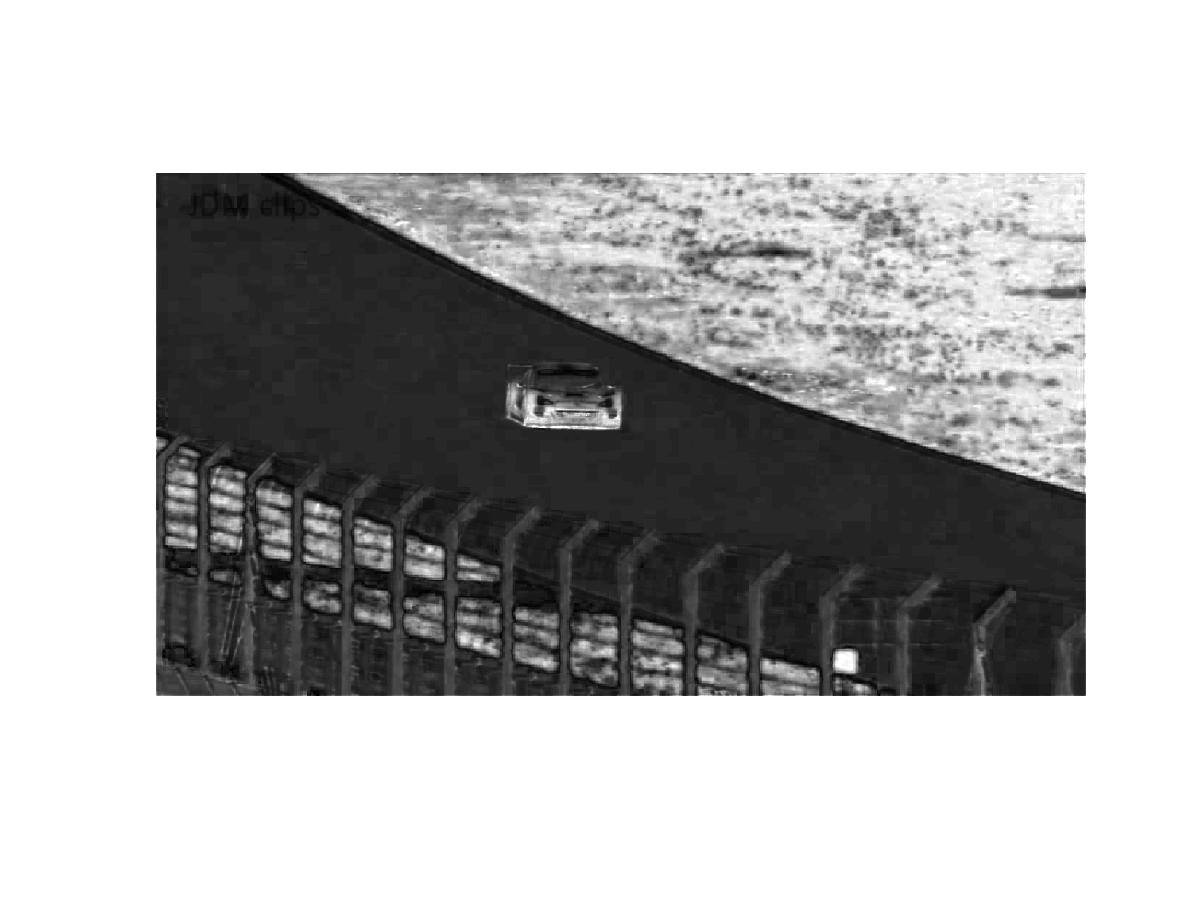
\includegraphics[width=0.48\linewidth]{generated/hsv_s}
}
\subfigure[Value]{
  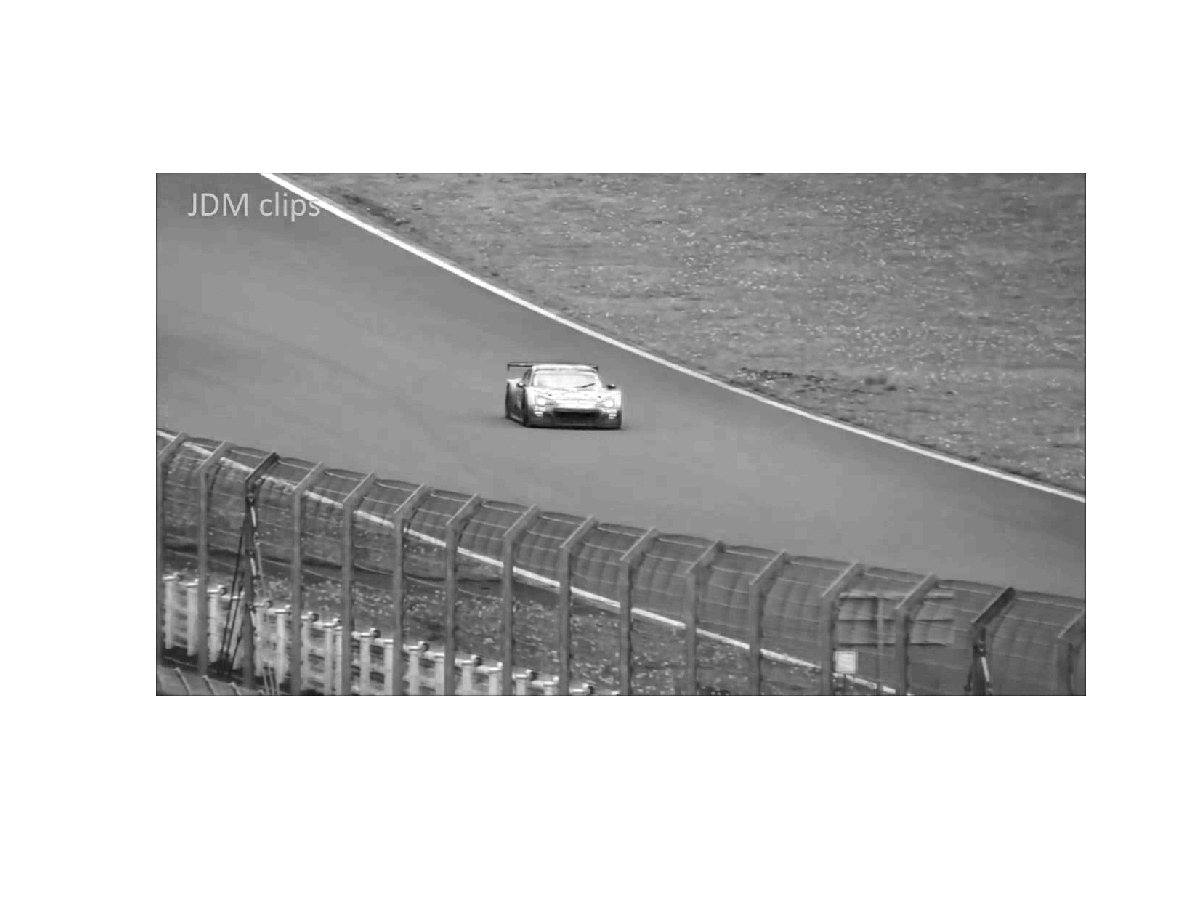
\includegraphics[width=0.48\linewidth]{generated/hsv_v}
}
\caption{Komponenten des HSV-Bildes}
\label{fig:1-1}
\end{figure}

Abbildung \ref{fig:1-1} zeigt deutlich, warum es {\bf nicht} sinnvoll ist, das Histogramm naiv aus den \emph{Hue}-Werten zu konstruieren: die Werte des Autos und der Straße sind zu ähnlich. Wo Bradski eine Filterfunktion vorschlägt, die vor Allem Pixel mit niedriger \emph{Value} filtert, erscheint hier das Filtern nach \emph{Satuation} sinnvoll: in dieser Dimension unterscheiden sich Auto und Straße deutlich.

Der vorliegenden Implementierung kann zur Berechnung des \emph{Hue}-Bildes eine Fehlerfunktion übergeben werden. Für den vorliegenden Fall wurde eine Fehlerfuktion gewählt die alle Pixel $(x,y)$ mit $sat((x,y))\le 0.2$ filtert. Hieraus ergeben sich das in Abbildung \ref{fig:1-2} gezeigte \emph{Hue}-Bild mit zugehörigem Histogramm.

\begin{figure}[!htpb]
\centering
\subfigure[Hue]{
  \raisebox{1cm}{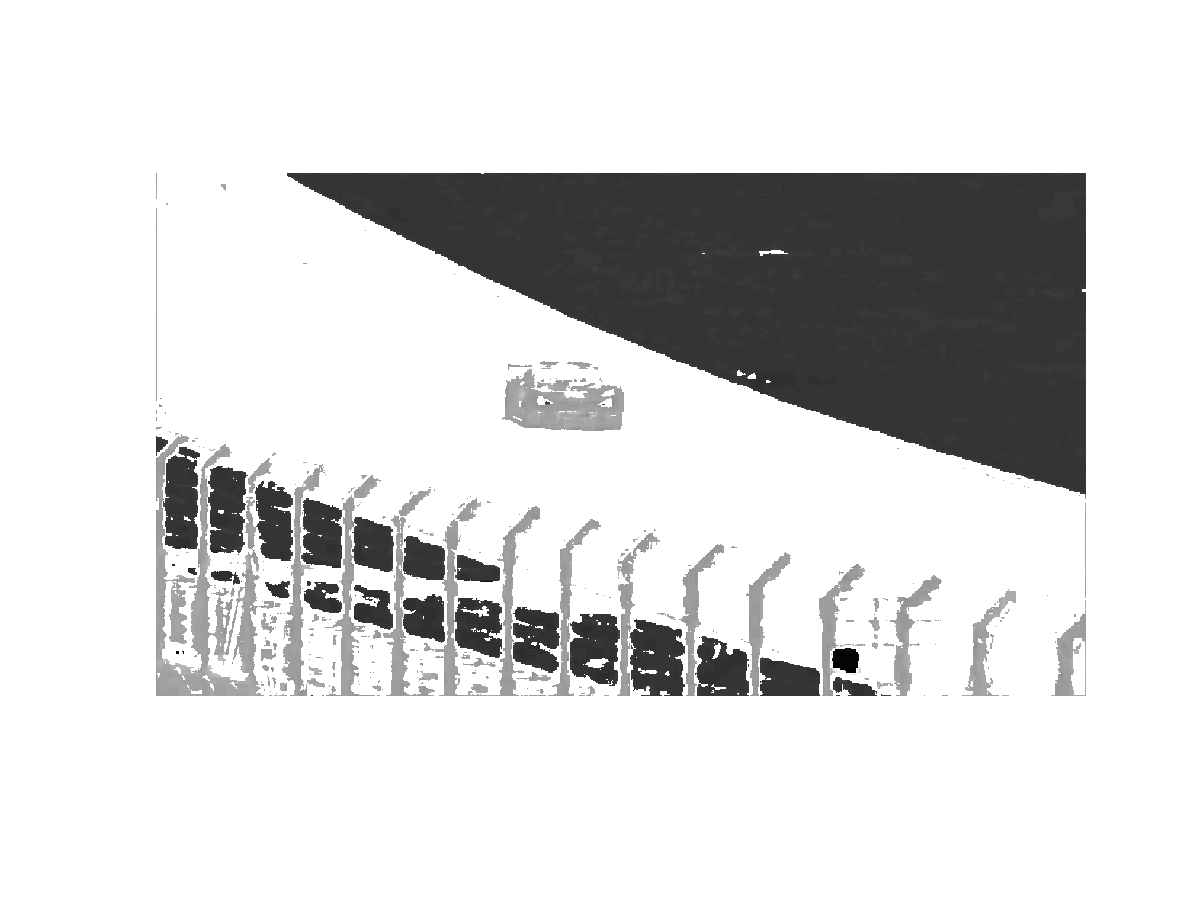
\includegraphics[width=0.48\linewidth]{generated/img_hue}}
}
\subfigure[Histogramm]{
  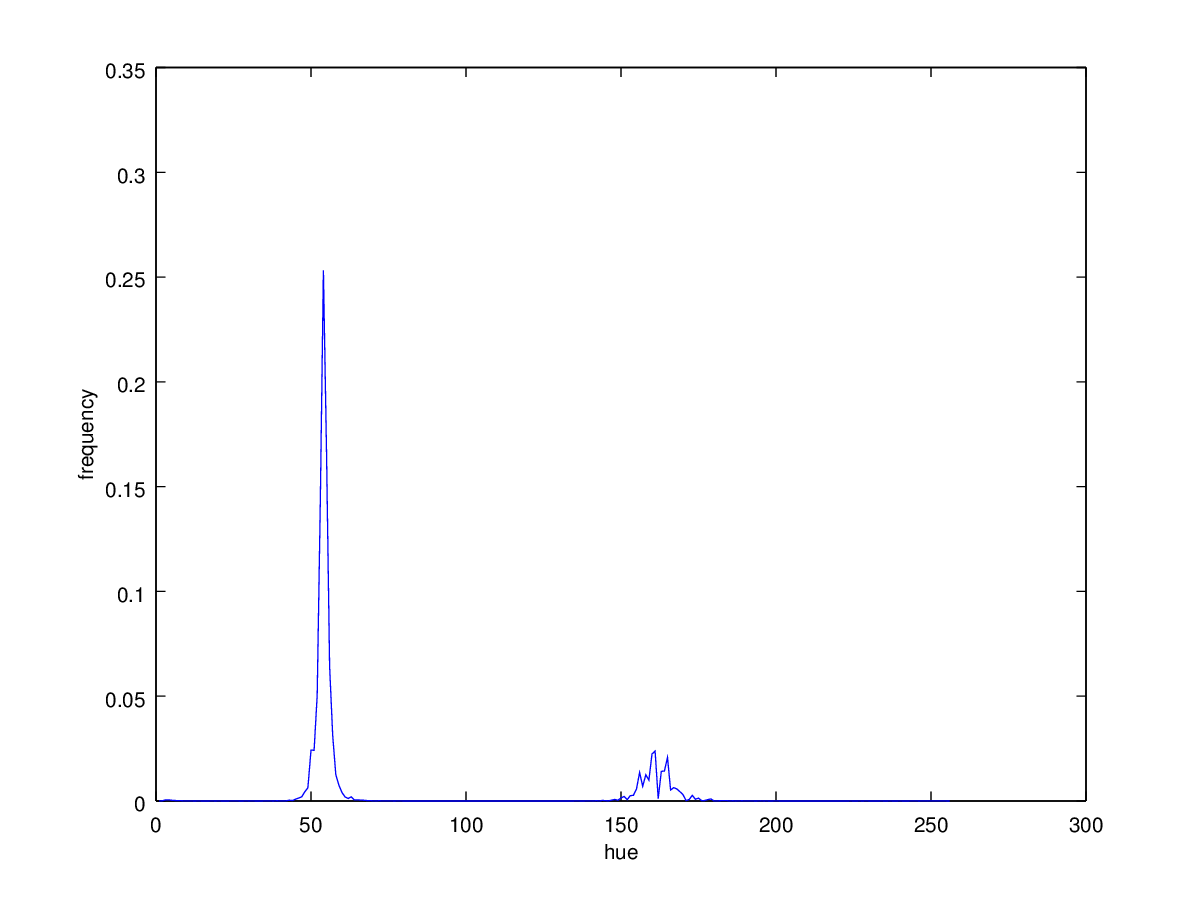
\includegraphics[width=0.48\linewidth]{generated/hist_img}
}
\caption{Mit Fehlerfunktion gefiltertes Bild}
\label{fig:1-2}
\end{figure}

\subtask{1.2}
\emph{und für den Ausschnitt $(x,y)=(460, 260)$ bis $(660,360)$}

Siehe Abbildung \ref{fig:1-3}. Der Ausschnitt ist einen Tick kleiner als angegeben.

\begin{figure}[!htpb]
\centering
\subfigure[RGB]{
  \raisebox{1cm}{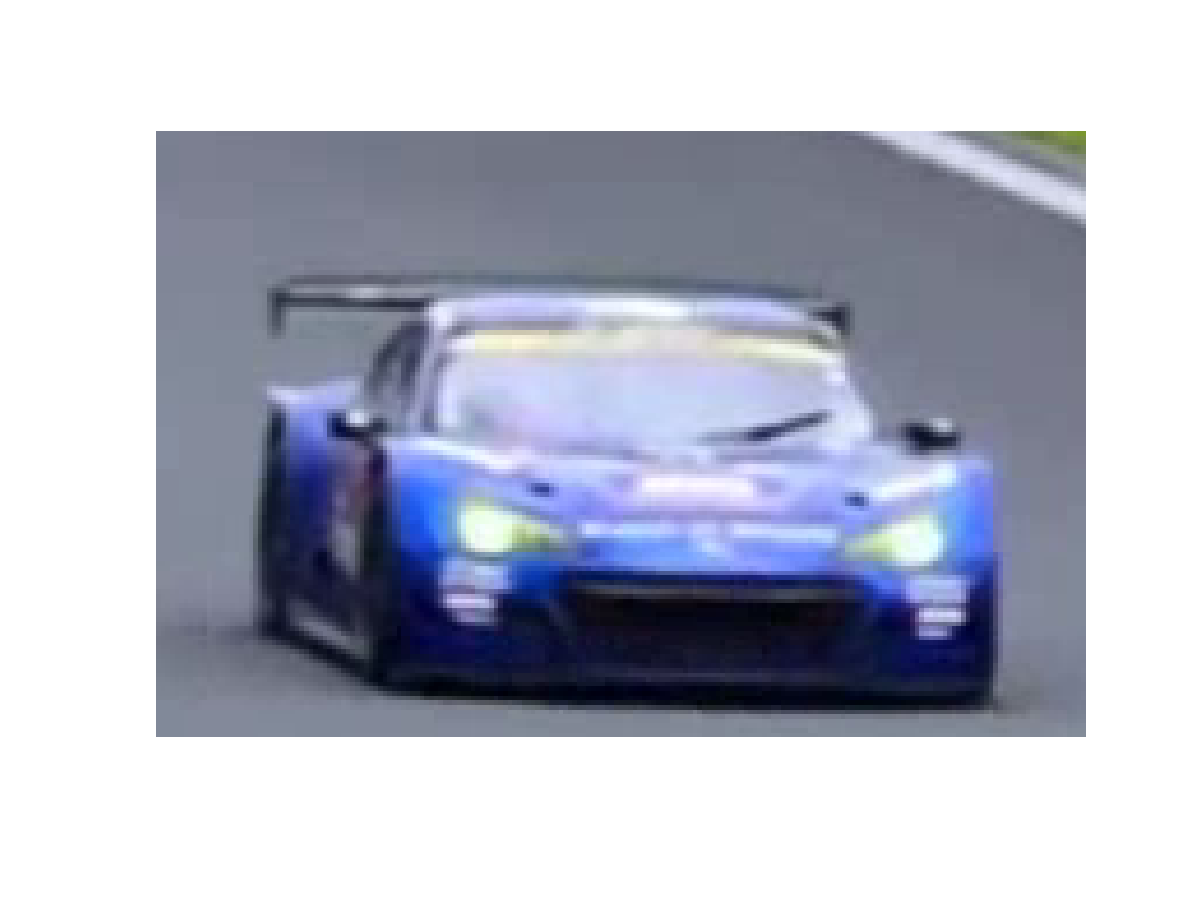
\includegraphics[width=0.48\linewidth]{generated/sub}}
}
\subfigure[gefiltertes Hue-Histogramm]{
  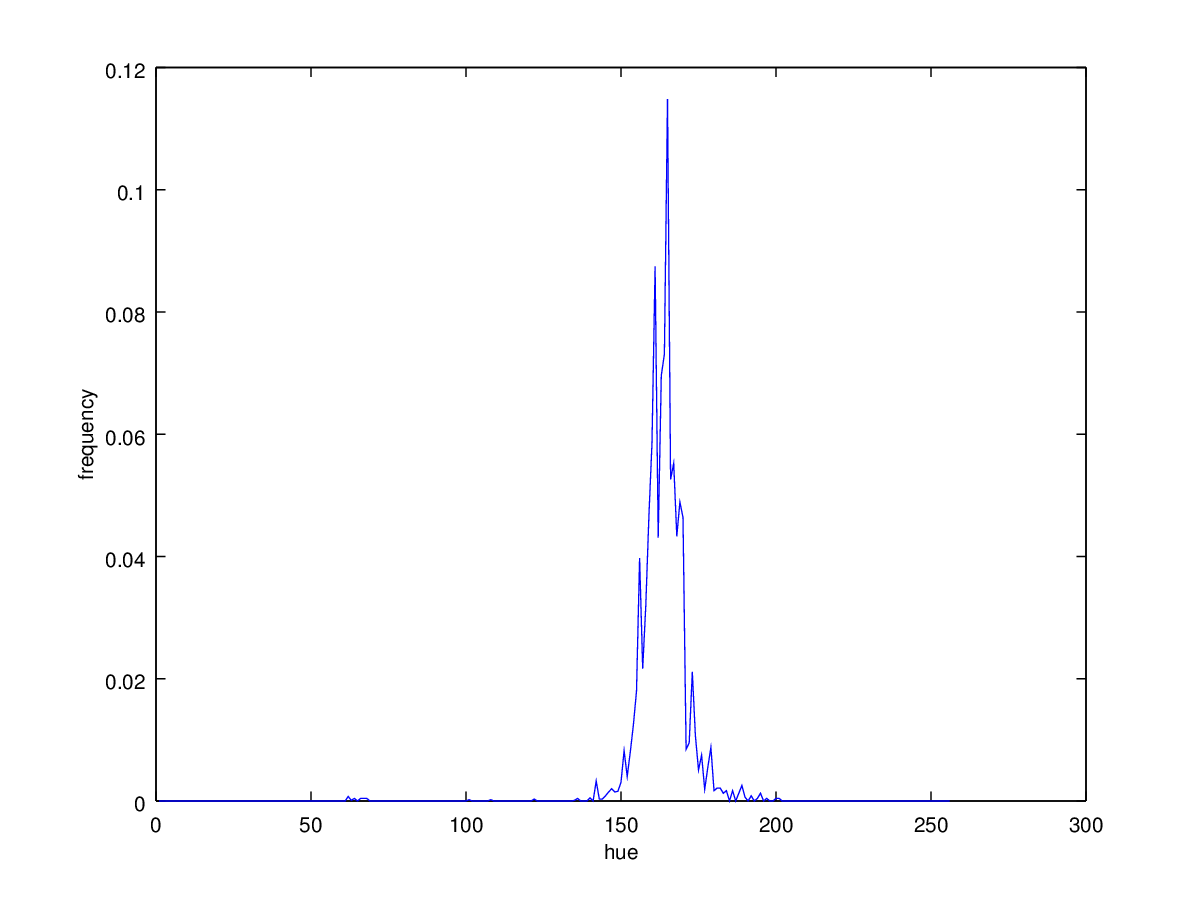
\includegraphics[width=0.48\linewidth]{generated/hist_sub}
}
\caption{Ausschnitt}
\label{fig:1-3}
\end{figure}
\end{task}

\begin{task}{CAMSHIFT}
\item[]\emph{- Lies das paper: \url{http://opencv.jp/opencv-1.0.0_org/docs/papers/camshift.pdf}\\
- implementiere eine Methode, die Dir - gegeben ein Hue-Histogramm - die Objekt-Wahrscheinlichkeitsverteilung für ein neues Bild berechnet (1)\\
- wähle aus dem angehängten Video ''racecar.avi'' ein Einzelbild (2)\\
- wende (1) für das Objekthistogramm aus Abgabe 1.2 auf (2) an und stelle das Ergebniss dar}

Aus dem Histogramm des gefilterten Hue-Bildes des Ausschnitts wird die Wahrscheinlichkeits-LUT erzeugt. Lookupen der Hue-Werte des Originalbildes (gefiltert) in dieser Tabelle liefert das Wahrscheinlichkeitsverteilungsbild in Abbildung \ref{fig:2-1}.

\begin{figure}[!htpb]
\centering
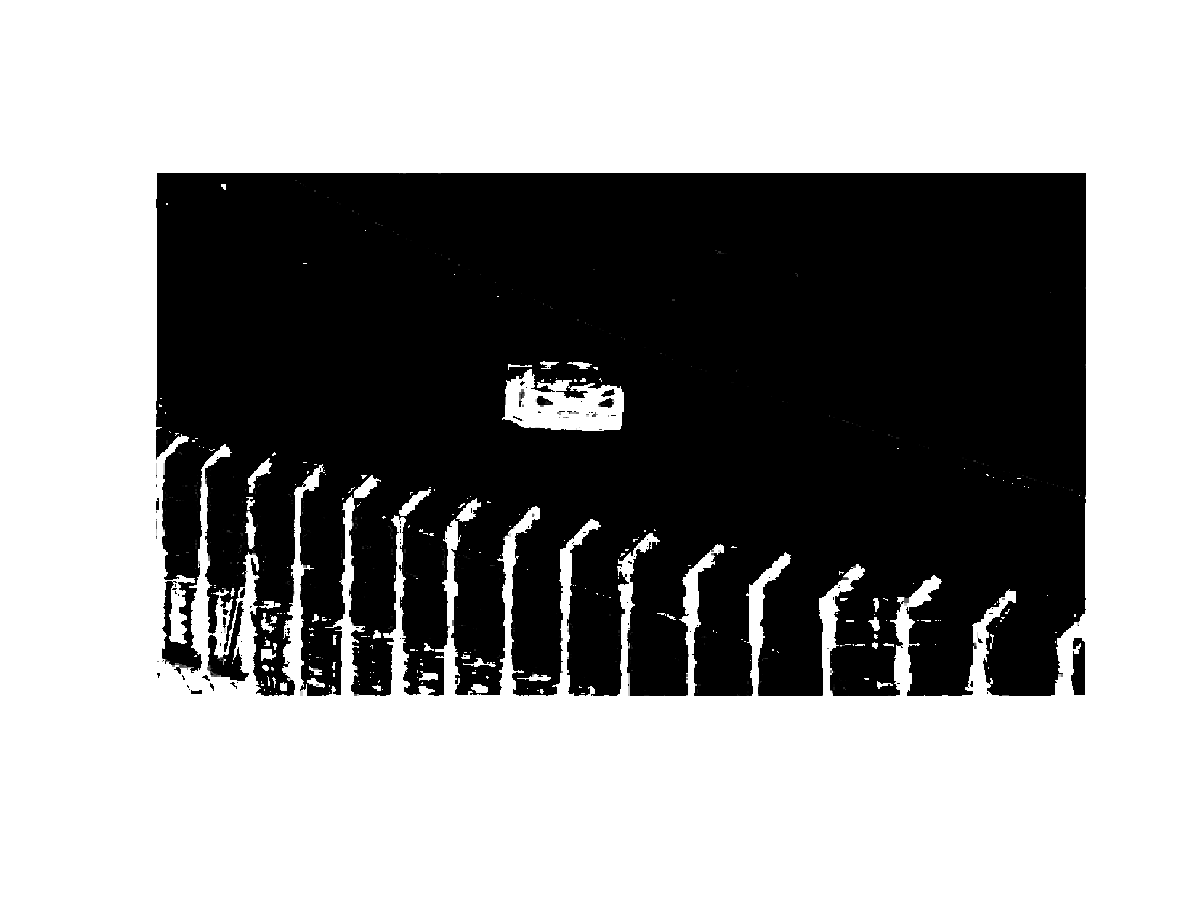
\includegraphics[width=0.7\linewidth]{generated/img_prob}
\caption{Wahrscheinlichkeitsverteilung}
\label{fig:2-1}
\end{figure}

Man kann hier bereits erahnen, dass die Differenzierung zwischen den ''Streben'' vorne im Bild und dem Auto nicht gut ist. Im Rahmen eines Übungszettels erscheint das hinnehmbar - grundsätzlich wäre aber eine ausgefeiltere Fehlerfunktion an dieser Stelle wünschenswert.

Mit der zuvor produzierten LUT können nun Einzelbilder aus dem avi analysiert werden: hierfür wird zunächst eine beliebige Fenstergröße angenommen, MEANSHIFT durchgeführt (mit Wahrscheinlichkeitsverteilung, LUT, und Fensterparametern), eine neue Fenstergröße berechnet und diese für das nächste Einzelbild gespeichert.

Das Berechnen einer neuen Fenstergröße ist hierbei nicht trivial und wird von Bradski für den konkreten ''Fleisch''-Fall beschrieben. Für das Auto gilt dieser nicht da:\\
- für das Auto kein sinnvoller Roll-Winkel gemessen werden kann\\
- sich die Aspect-Ratio (die Bradski als konstant annimmt) deutlich ändern kann

In der vorliegenden Implementierung kann an CAMSHIFT eine Funktion zur Berechnung der neuen Fenstergröße übergeben werden, für die als Parameter die Bild-Momente $0.-2.$ Grades $m_{00},m_{10},m_{01},m_{02},m_{20}$ zur Verfügung stehen. Experimentell hat sich im vorliegenden Fall eine lineare Funktion von $\sqrt{m_{00}}$ als hinreichend gut erwiesen. Zur Berechnung der neuen Aspect-Ratio $ar$ wird stets
$$ar=m_{20}\cdot\left(\frac{m_{00}}{m_{10}}^2\right)/m_{02}\cdot\left(\frac{m_{00}}{m_{01}}\right)^2$$
berechnet. Die Abbildung \ref{fig:2-2}-\ref{fig:2-3} zeigen das Resultat bei Anwendung des Algorithmus auf einige aufeinanderfolgende Frames (bei einer Framerate von 1).

\begin{figure}[!htpb]
\centering
\subfigure[Frame 1]{
  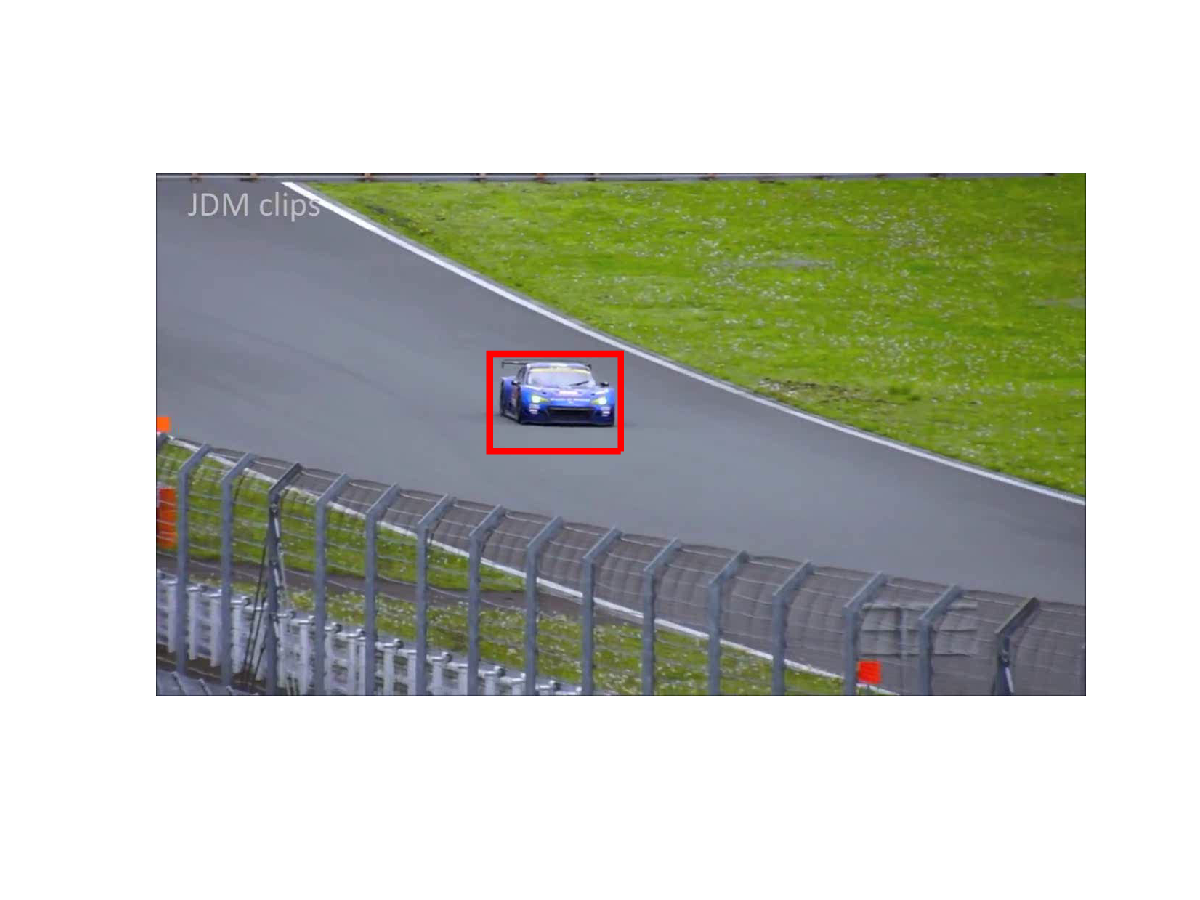
\includegraphics[width=0.48\linewidth]{generated/frame_01}
}
\subfigure[Frame 2]{
  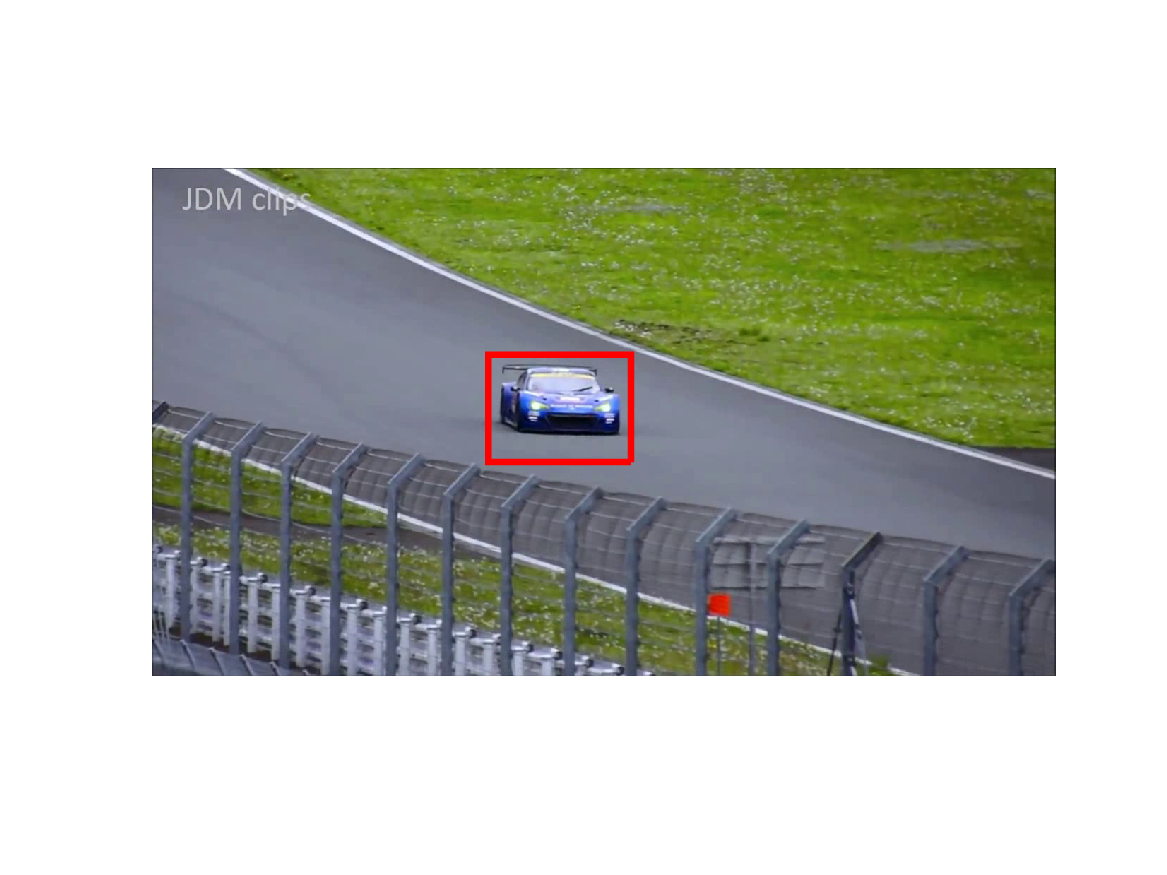
\includegraphics[width=0.48\linewidth]{generated/frame_02}
}
\subfigure[Frame 3]{
  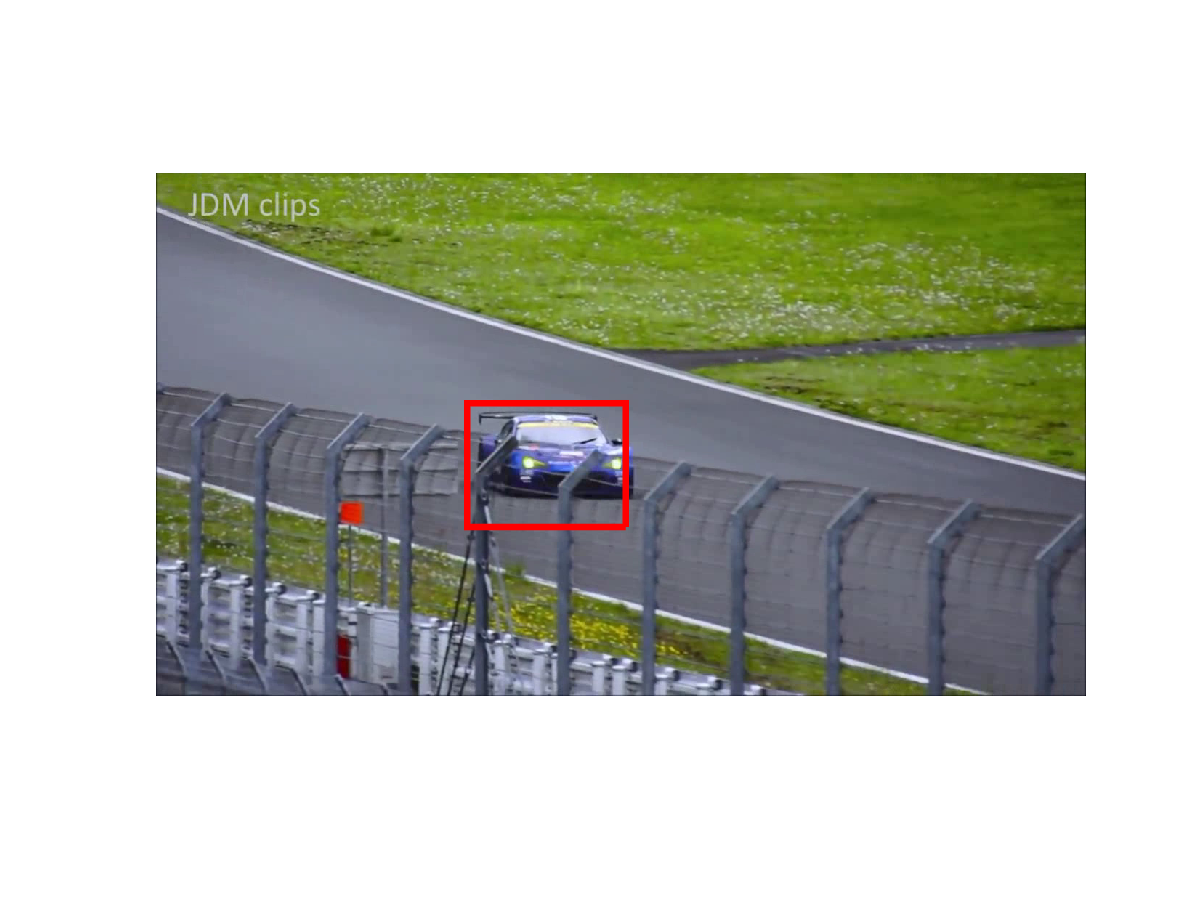
\includegraphics[width=0.48\linewidth]{generated/frame_03}
}
\subfigure[Frame 4]{
  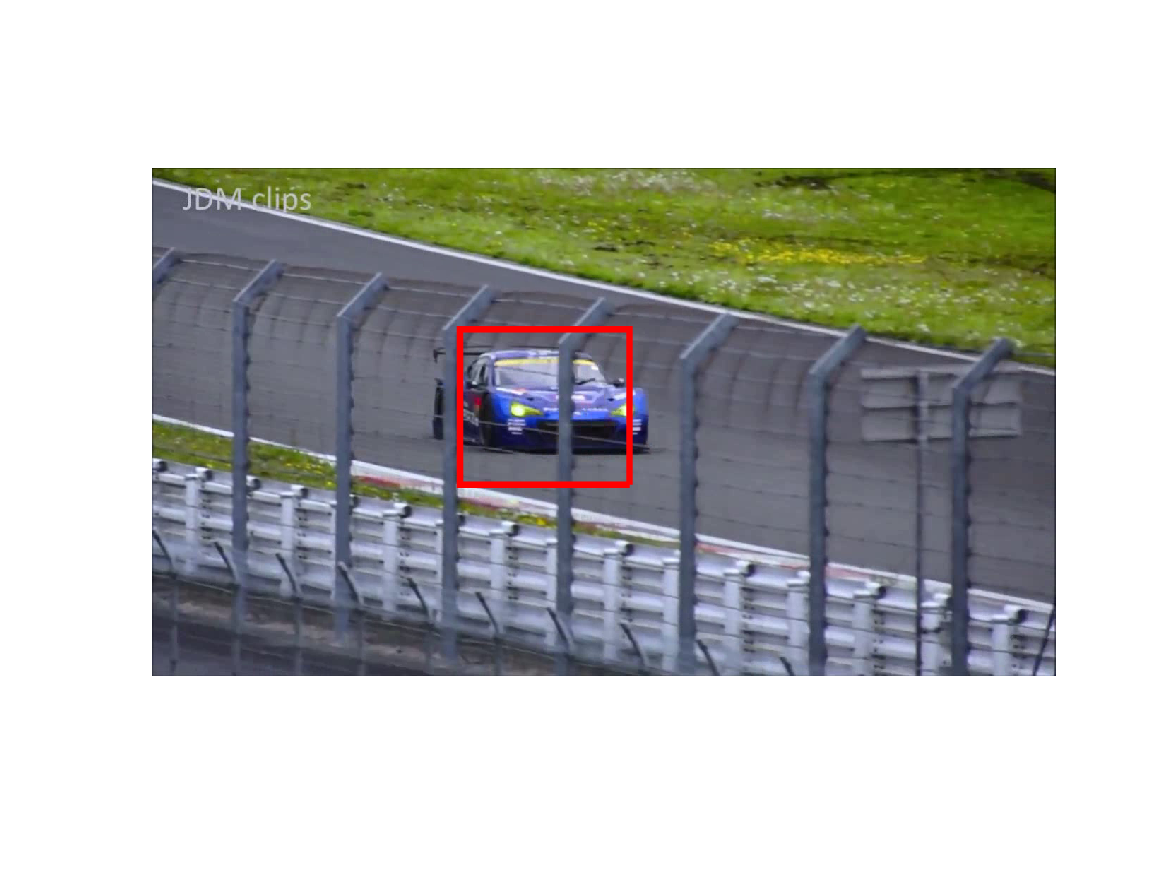
\includegraphics[width=0.48\linewidth]{generated/frame_04}
}
\subfigure[Frame 5]{
  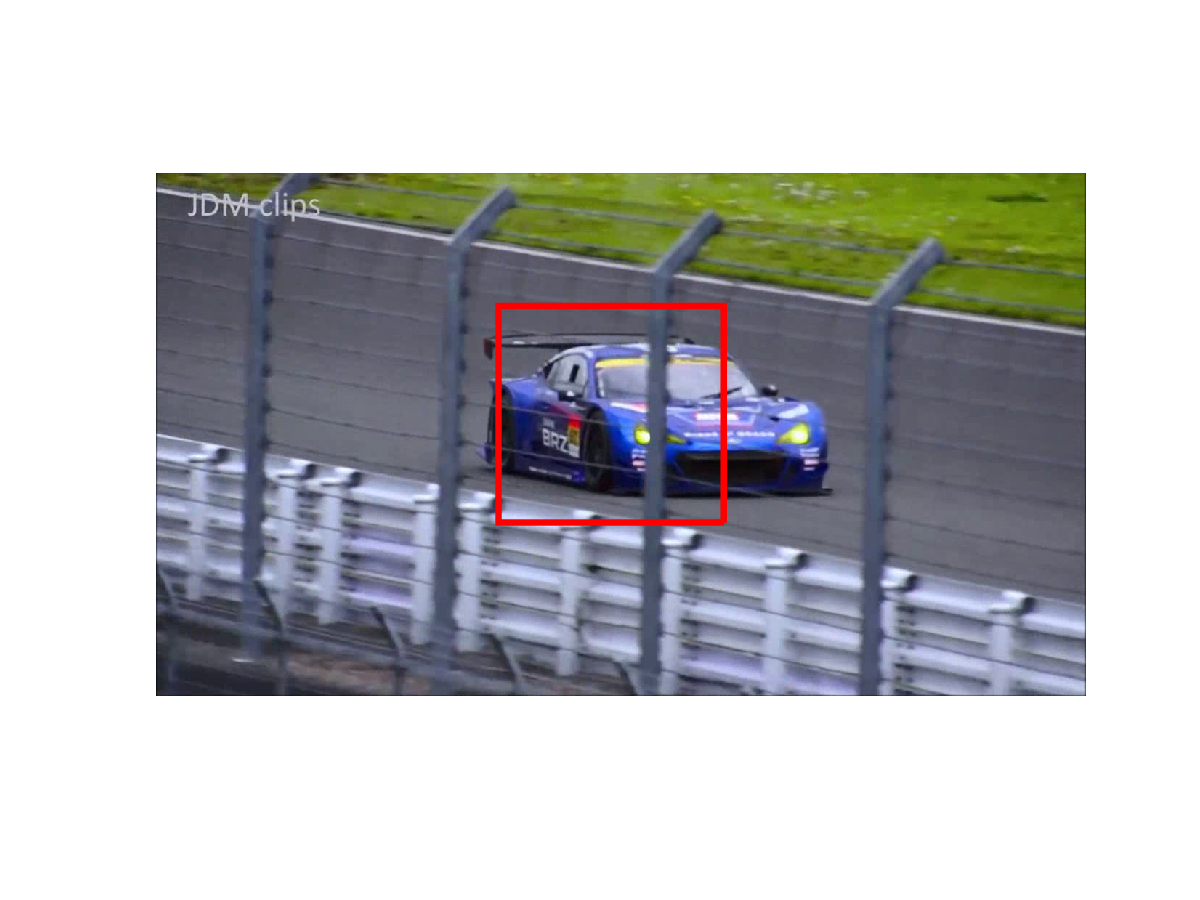
\includegraphics[width=0.48\linewidth]{generated/frame_05}
}
\subfigure[Frame 6]{
  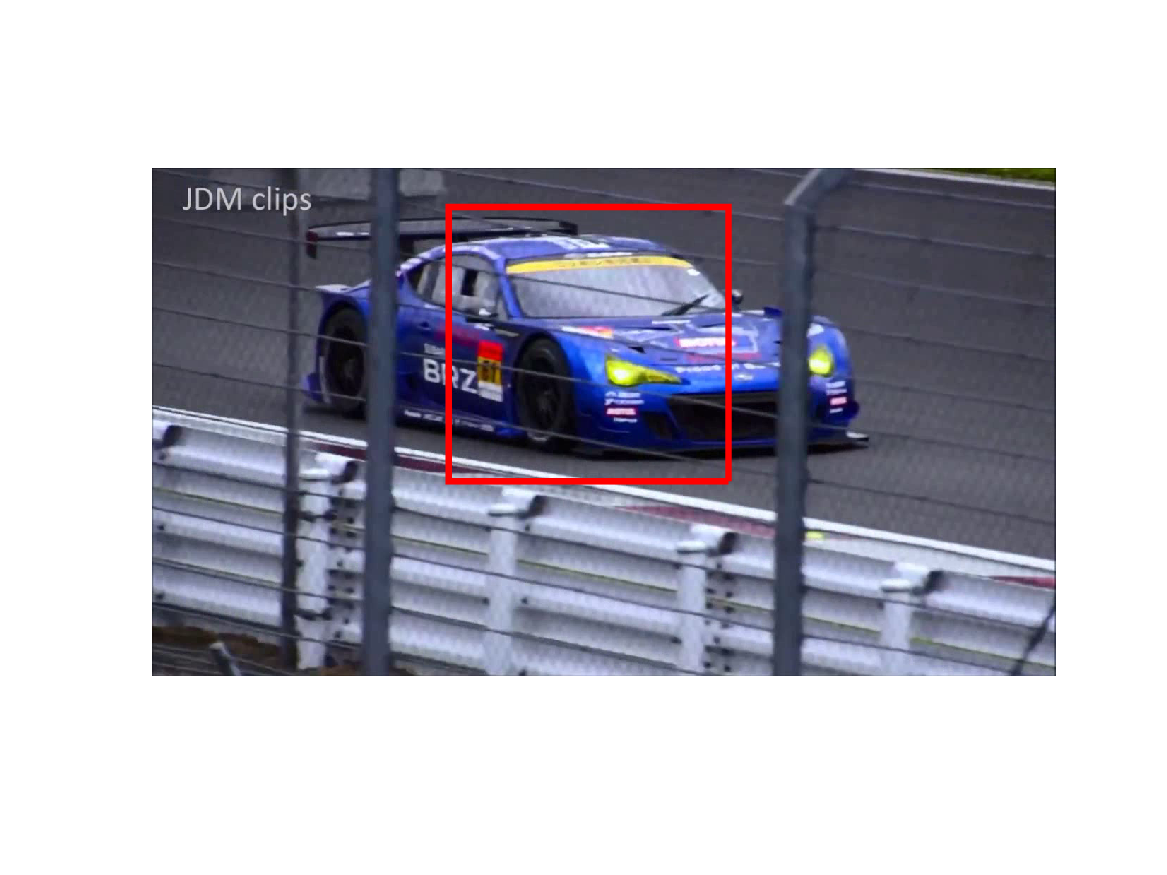
\includegraphics[width=0.48\linewidth]{generated/frame_06}
}
\caption{Resultat (1)}
\label{fig:2-2}
\end{figure}

\begin{figure}[!htpb]
\centering
\subfigure[Frame 7]{
  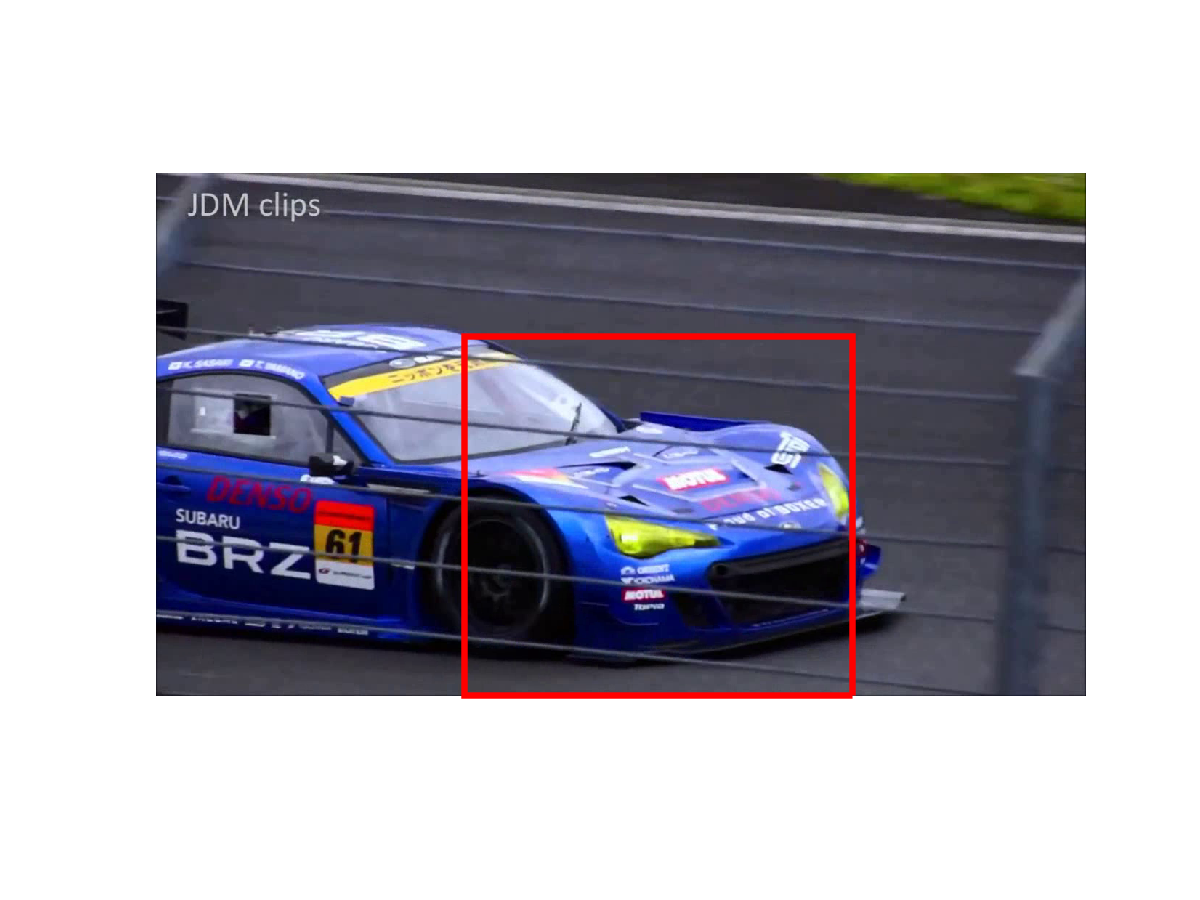
\includegraphics[width=0.48\linewidth]{generated/frame_07}
}
\subfigure[Frame 8]{
  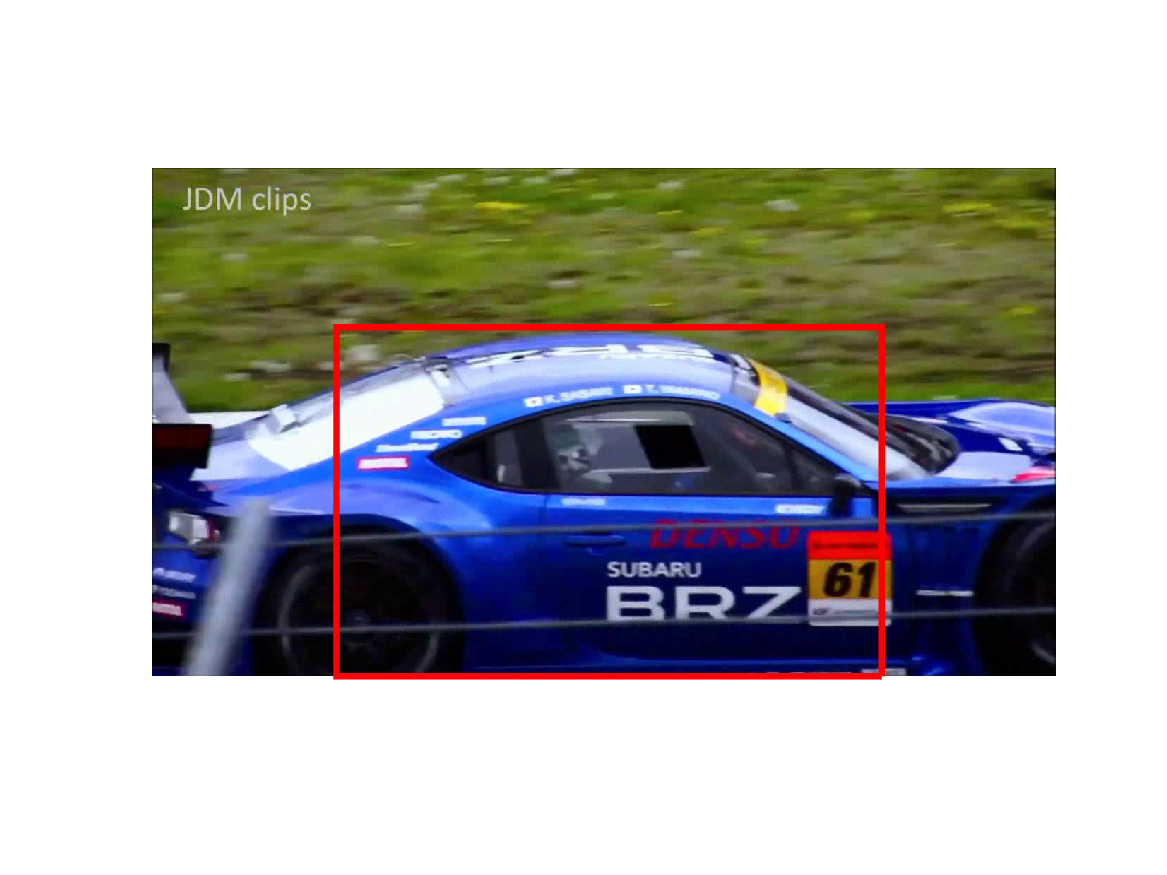
\includegraphics[width=0.48\linewidth]{generated/frame_08}
}
\subfigure[Frame 9]{
  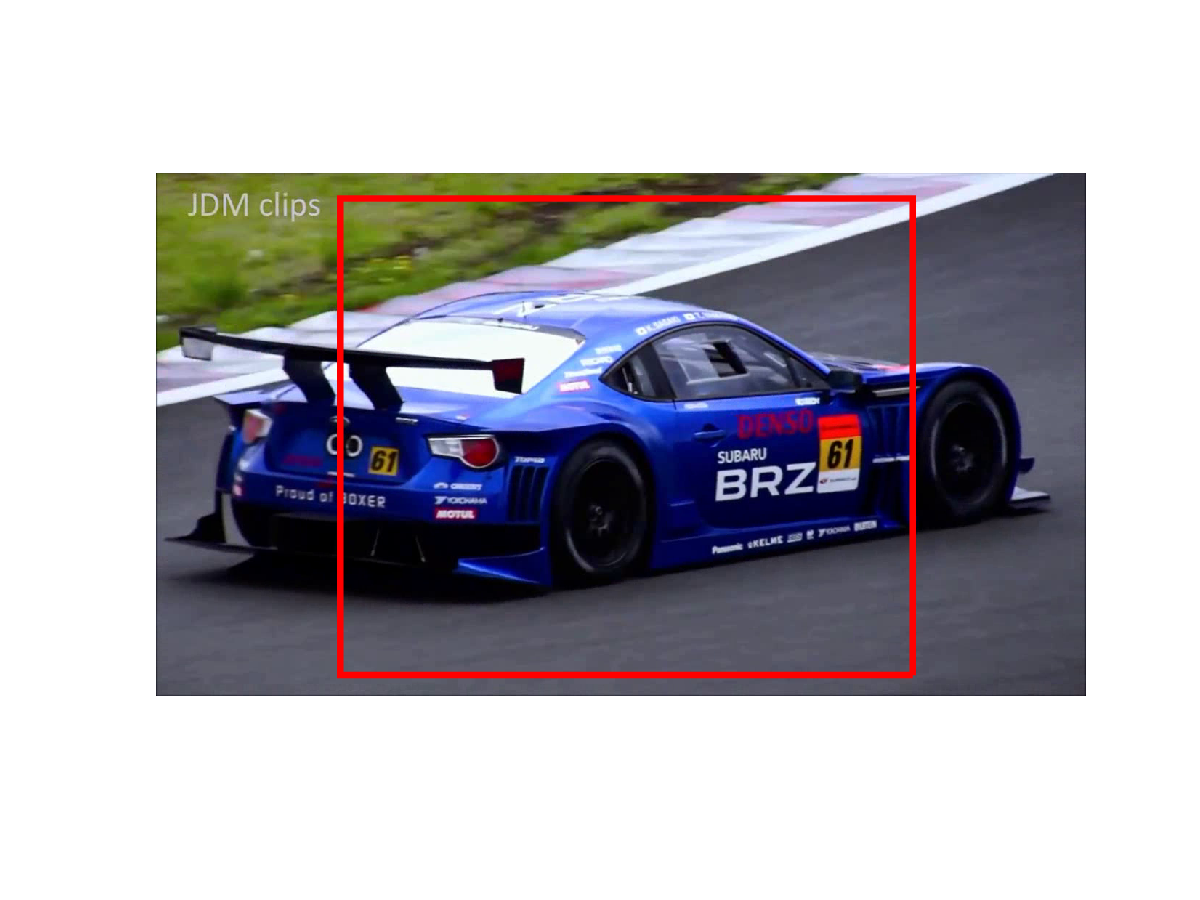
\includegraphics[width=0.48\linewidth]{generated/frame_09}
}
\subfigure[Frame 10]{
  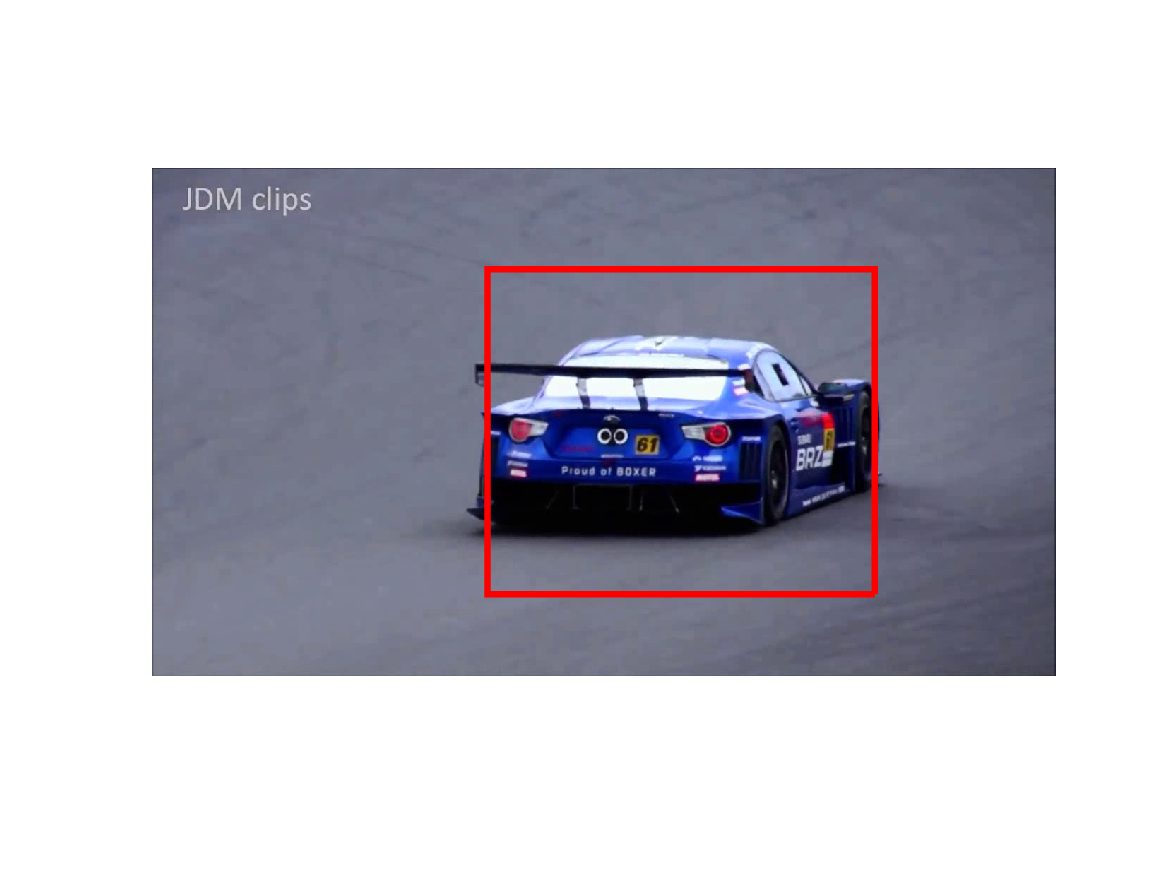
\includegraphics[width=0.48\linewidth]{generated/frame_10}
}
\subfigure[Frame 11]{
  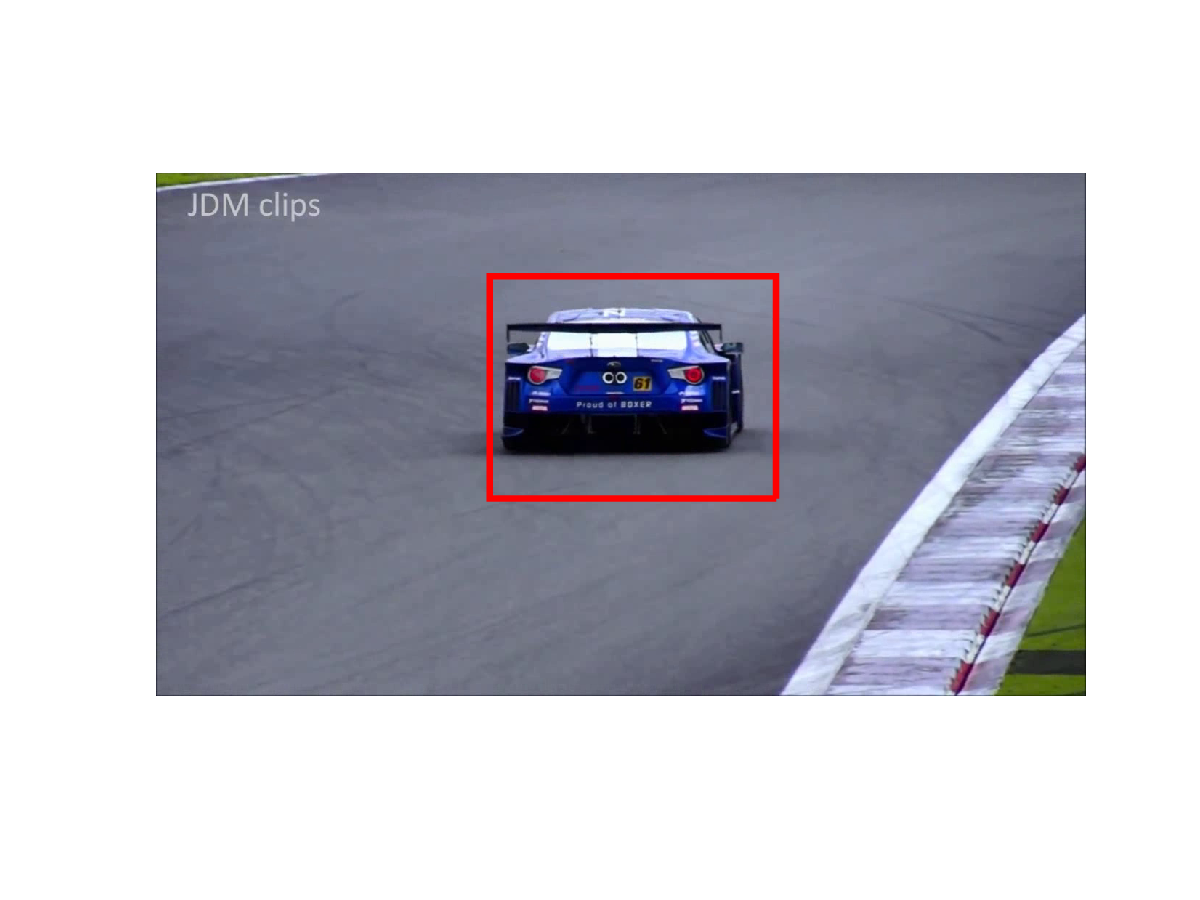
\includegraphics[width=0.48\linewidth]{generated/frame_11}
}
\caption{Resultat (2)}
\label{fig:2-3}
\end{figure}
\end{task}
\end{document}